\documentclass[11pt,a4paper]{article}

\usepackage[parfill]{parskip}
\usepackage{subfig}
\usepackage{amsmath}
\usepackage{makeidx}
\usepackage{graphicx}
\usepackage[bibstyle=numeric, citestyle=numeric-comp, backend=bibtex, sorting=none, url=false, isbn=false, eprint=false, autocite=superscript]{biblatex}
\usepackage{multicol}
\usepackage{letltxmacro}
\usepackage{listings}
\usepackage[english]{isodate}
\usepackage[colorlinks=true,hyperfootnotes=false,citecolor=blue]{hyperref}

\addbibresource{Report_Papers.bib}

\LetLtxMacro{\oldsqrt}{\sqrt} % makes all sqrts closed
\renewcommand{\sqrt}[1][]{%
  \def\DHLindex{#1}\mathpalette\DHLhksqrt}
  \def\DHLhksqrt#1#2{%
    \setbox0=\hbox{$#1\oldsqrt[\DHLindex]{#2\,}$}\dimen0=\ht0
    \advance\dimen0-0.2\ht0
    \setbox2=\hbox{\vrule height\ht0 depth -\dimen0}%
    {\box0\lower0.71pt\box2}}

    \makeatletter
    \newenvironment{tablehere}
    {\def\@captype{table}}
    {}

    \newenvironment{figurehere}
    {\def\@captype{figure}}
    {}
    \makeatother

    \title{Automatic Fingerprint Recognition}
    \author{Benjamin May \& Edward Wastell}
	\date{}

    \begin{document}
    \maketitle

    \begin{abstract}
      Fingerprint analysis has many applications, from biometric identification to crime scene investigation. If fingerprints are to be used, a method for quickly and accurately determining if two fingerprints come from the same person. Many approaches have been proposed, but minutia extraction, where information about where the ridges of a fingerprint terminate has had the most success. In this articles, we shall explore a method for investigating such features by using an algorithm that follows ridges by detecting the rate of change of the greylevel, without any prior processing. We apply such methods to some sample images similar to real world fingerprints, and discuss the usefulness of such an approach.
    \end{abstract}

    \begin{multicols}{2}

\section{Introduction}
	Fingerprints have been used to identify people since the 19\textsuperscript{th} century and have been used in criminal investigations since about that time. More recently fingerprints have been used as biometric markers used in boarder control, library stock control and computer and building access control systems. The need for a robust automatic fingerprint recognition system is obvious.

        If fingerprints are to be used in a modern setting, a method to rapidly compare different fingerprints is needed. This obviously requires some form of algorithm that can be run on a computer. The naive approach would be to simply calculate the total piecewise difference between two different images; if this value is below a certain threshold we can say the images are the same and hence belong to the same person. However, this system would have almost no tolerance for error. If the image was distorted, captured with different method or machine, or the finger was simply rotated this will give a false mismatch. Conversely, if the image is sufficiently low quality images would look more similar and false matches would be common. In theory, there is an operation that would process the image in such a way that this would be possible, it turns out that there is a far simpler way.

        Fingerprints can be classified by a collection of features called minutia\supercite{ANSI}. These are features of how the individual ridges of the fingerprint pattern behaves. Any point where a line halts and is not at the edge of a region is a termination, and any point where a ridge splits in two is a bifurcation. By knowing the location and nature of all minutia of a fingerprint it is thought to be possible say whether two fingerprints are the same: this fact has not been proved but no instance of two people having the same set of minutia. There are a number of advantages to comparing a list of minutia as opposed to doing the same with a collection of images, the first of which is space. Although modern computers can store many high resolution images, a relatively small list of points is several orders of magnitudes smaller. The second reason is accuracy. It is unlikely that two pictures of fingerprints are exactly the same - there are many ways small errors in image acquisition can occur. If using exact picture matching, some on the fly processing must happen to get different images to be comparable, which can loose some information. Lastly, minutia matching should be faster.


        Traditionally, fingerprint analysis consisted of first processing the image in some way, usually either binarisation\supercite{Moayer} or line thinning. Methods like this have two major drawbacks. Firstly, such alterations to the image can be computationally expensive and therefore take a considerable amount of time for large images, which is a serious problem when used in real time applications. Secondly, non-reversible image manipulation can lead to destruction of information about the fingerprint. In this article, we aim to implement a method for following a series of ridges, such as those found in fingerprints, and show how this could be applied to minutia extraction.



\section{Theory and Implementation}
        The method used in the article does not rely on prior image manipulation. It works by think of the image as a three dimensional object, with the greylevel of time image being the height in the Z-direction. The tangent of this object is then calculated at the position of each pixel in the image. A line can then be traced along the image by taking steps in the direction orthogonal to these tangents. By building up such lines from different starting points in the image, we can classify the entirety of the fingerprint. The two types of minutia we are looking for can be found from this complete classification. Where a line ends without touching another line or the edge of the image is a termination and points where one line hits the middle of another are bifurcations. The work in this article is based on work by Donahue and Rokhlin\supercite{Donahue} and expanded by Maio and Maltone\supercite{Maio}.


	\subsection{Point Normal Direction}
\begin{figure*}
\centering
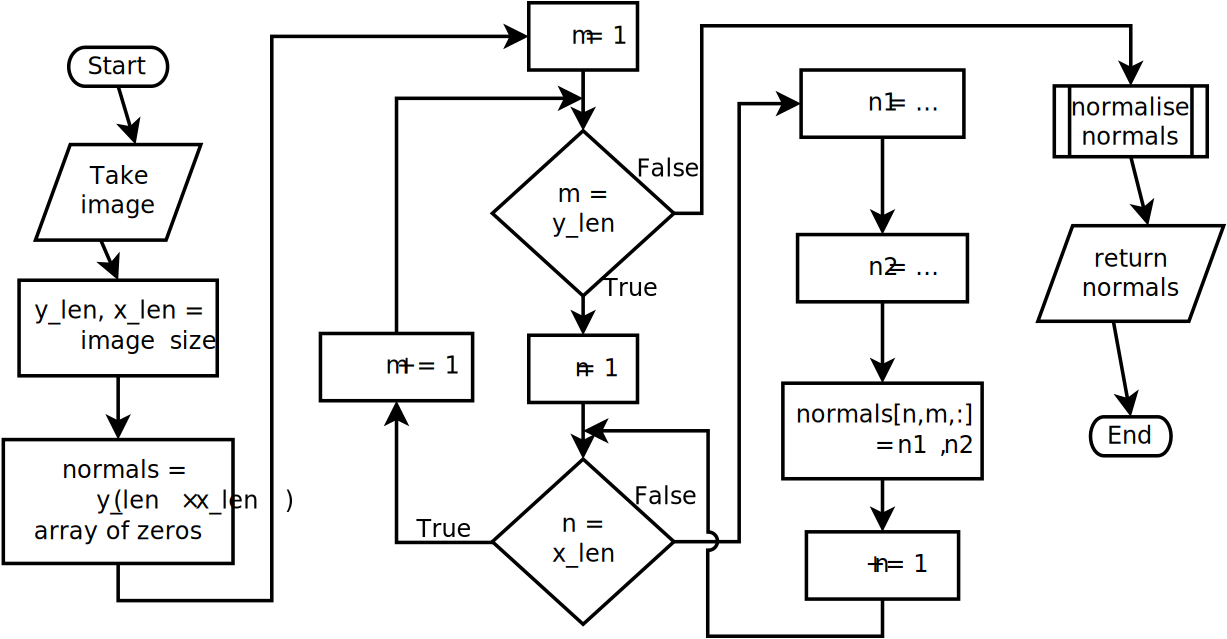
\includegraphics[width = \textwidth]{PND}
\caption{Flow chart of the PND function as implemented.}
\label{fig:PND-alg}
\end{figure*}


		The point normal function works by taking four mutually adjacent points (\textit{i.e.} a $2 \times 2$ array of pixels) and fitting a plane to them. If the greylevel at the pixel $(x_k, y_k)$ is denoted $h_k$ and the level from the fitted plane is denoted $p_k$ then the plane fitting part of the function can be seen as minimising the following expression:

		\begin{equation}
			\min_{n_1, n_2, c} \sum_k |h_k - p_k|^2
		\end{equation}
		
		Which in matrix form can be expressed as:

		\begin{equation}
			\begin{vmatrix}
			\begin{pmatrix}
			h_1 \\
			h_2 \\
			h_3 \\
			h_4
			\end{pmatrix}
			-
			\begin{pmatrix}
			-x_1 & -y_1 & 1 \\
			-x_2 & -y_2 & 1 \\
			-x_3 & -y_3 & 1 \\
			-x_4 & -y_4 & 1
			\end{pmatrix}
			\begin{pmatrix}
			n_1 \\
			n_2 \\
			c
			\end{pmatrix}
			\end{vmatrix}^2
		\end{equation}

		Where $n_1$, $n_2$ and $c$ are the $x$, $y$ and $z$ components of the surface normal respectively. This is a simple least-squares minimisation and after some rearranging we obtain the following expressions for the optimum surface normal:

		\begin{equation}
		\begin{split}
			n_1 = \frac{-h_1 + h_2 + h_3 - h_4}{4} \\
			n_2 = \frac{-h_1 - h_2 + h_3 + h_4}{4} \\
			c = \frac{h_1 + h_2 + h_3 + h_4}{4}
		\end{split}
		\end{equation}

		Since we are only concerned with the components in the $x,y$--plane the function implemented here doesn't bother calculating $c$ (figure \ref{fig:PND-alg}). Once all $2 \times 2$ neighbourhoods have been fitted the function returns $n_1$ and $n_2$ then terminates.

		As the NPD function needs a four points to fit a plane to the decision has to be made regarding how edges are handled. One possibility is to `wrap' the edges of the image around, effectively forming a torus --- this was not implemented here because it would mean that for two edges the values of $n_1$ and $n_2$ would depend on greylevels from the other two edges. The second possibility (implemented here) is to make the output array smaller by 1 pixel in both dimensions, so if the original image is $n \times m$ pixels the array of normals is $(n-1) \times (m-1)$. From figure \ref{fig:PND-alg} it can be seen that the PND function implemented here loses the top and right hand pixels.

	\subsection{Averaged Tangent Direction}
        \begin{figure*}
        \centering
        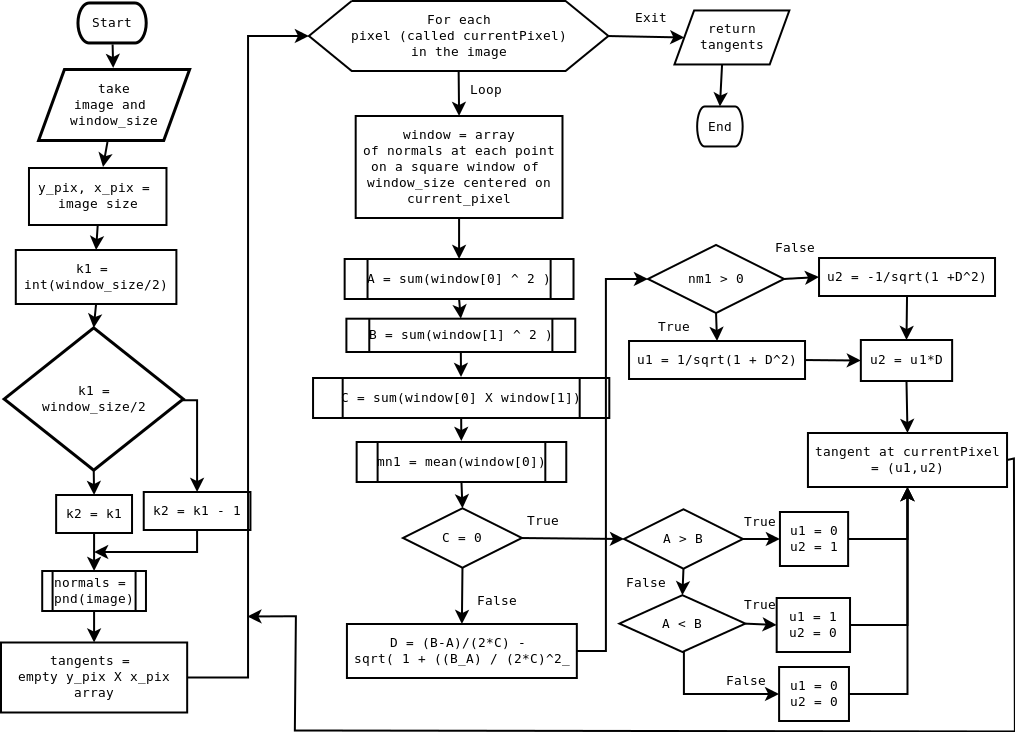
\includegraphics[width = \textwidth]{ATD}
        \caption{Flow chart of the ATD function as implemented.}
        \label{fig:ATD-alg}
      \end{figure*}
		The ATD function calculates the $x,y$--plane tangent that best fits with the surface normals generated by the PND function in a given $n \times n$ neighbourhood. This has the effect of smoothing out (plane normal angle) noise but, as with analogous smoothing operations, can obscure features with a size comparable to that of the kernel chosen. The fitting is a least squares minimisation of the row-by-row dot product:

		\begin{equation}
		\begin{split}
			\min_{u_1, u_2} \sum_k |(n_{1,k}, n_{2,k}) \cdot (u_1, u_2)|^2 \\
			= U(u_1, u_2)
		\end{split}
		\end{equation}

		Where $n_{1,k}$ is the $k$\textsuperscript{th} $n_1$ value as defined above \textit{e.t.c.} and $(u_1, u_2)$ is the normalised fitted vector. If we define the following:

		\begin{equation}
		\begin{split}
			A = \sum_k (n_{1,k})^2 \\
			B = \sum_k (n_{2,k})^2 \\
			C = \sum_k n_{1,k} n_{2,k}
		\end{split}
		\end{equation}

		then we can express $U(u_1, u_2)$ as

		\begin{equation}\label{eq:U_mat}
		\begin{split}
			U(u_1, u_2) = \\ (u_1, u_2)
			\begin{pmatrix}
			A & C \\
			C & B
			\end{pmatrix}
			\begin{pmatrix}
			u_1\\
			u_2
			\end{pmatrix}
		\end{split}
		\end{equation}

		The eigenvalues of the above $2 \times 2$ matrix, $\lambda_1$ and $\lambda_2$, are the maximum and minimum values of $U$ respectively. It is trivial to determine that the two eigenvalues are given by:

		\begin{equation}
		\begin{split}
			\lambda_1 = \frac{A + B + \sqrt{(A - B)^2 + 4C^2}}{4} \\
			\lambda_2 = \frac{A + B - \sqrt{(A - B)^2 + 4C^2}}{4}
		\end{split}
		\end{equation}

		With some further rearranging of equation \eqref{eq:U_mat} we find that:

		\begin{equation}\label{eq:ATD_u}
			u_1 = \sqrt{\frac{1}{1 + \left(\frac{\lambda_2 - A}{C}\right)^2}}
		\end{equation}

		\begin{equation}
			u_2 = u_1 \left(\frac{\lambda_2 - A}{C}\right)
		\end{equation}

		In implementing these equations several special cases have to be taken into account. The first special case is when $C = 0$, which would require dividing by zero. To cope with this case the function is set to test if $C = 0$ and if so the function will set $(u_1, u_2) = (1,0)$ or $(u_1, u_2) = (0,1)$ depending on weather $A < B$ or $B > A$ respectively. The second special case is  when $\lambda_1 = \lambda_2$, which the function tests for after determining if $C = 0$. In this case there is no optimum orientations thus $(u_1, u_2) = (0,0)$.

		A final problem with implementing equation \eqref{eq:ATD_u} is the fact that $u_1$ can only ever be positive. This ensures that in the $x$--direction one cannot distinguish between the two sides edges of a ridge. To solve this the function calculates the mean of the $n_1$ values then checks if this mean is negative and if so it makes $u_1$ negative.

	\subsection{The Ridge Follower}
		The ridge following system takes a slice (of width $2 \sigma + 1$ and height 1 pixel centred around pixel $(x_c, y_c)$) of the image, finds the peak of the ridge and moves to it, calculates the direction of the ridge ($\phi_c$) then moves forward by $\mu$ pixels before starting the process again (figure \ref{fig:ridge_follow_simpled}). In this manor the ridge follower follows the ridge, and since the function logs where it's been it's possible to determine where the minutiae are.

\begin{figurehere}
\centering
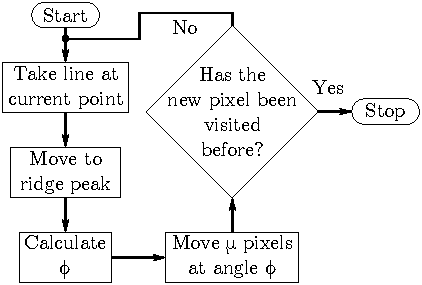
\includegraphics[width = 0.48\textwidth]{ridge_follow_simpled}
\caption{Simple version of the ridge following algorithm.}
\label{fig:ridge_follow_simpled}
\end{figurehere}

		Taking a line at a given point is simple enough: the current pixel, $(x_c, y_c)$, is the centre of the line and by simple trig the coordinates of the pixels that make up the line are

		\begin{equation}
		\begin{split}
			\begin{pmatrix}
			x_{l,k} \\
			y_{l,k}
			\end{pmatrix}
			= \\
			\begin{pmatrix}
			x_c \\
			y_c
			\end{pmatrix}
			+ (k - \sigma)
			\begin{pmatrix}
			\cos{(\phi_c + \pi/2)} \\
			\sin{(\phi_c + \pi/2)}
			\end{pmatrix}
		\end{split}
		\end{equation}

		where $x_{l,k}$ is $x$--coordinate of the $k$\textsuperscript{th} pixel of the line \textit{e.t.c.} and $k$ ranges from zero to $2 \sigma + 1$. Using these coordinates one can extract the relevant greylevels and plane normals.

		Identifying the peak of the ridge is somewhat involved if noise tolerance is needed. One method is to find the point midway between the two angles that are closest to the end of the lines. Another method is to try and smooth out the ridge to ensure that there is just one peak in it - by taking the average of a line in front of and behind the current point then convolving along the line with a Gaussian mask one can effectively find the `weak' maxima of the ridge. This weak maxima may not be the actual centre of the ridge but it should be near enough. In the algorithm employed here a more simplistic (and not as noise tolerant) method that simply finds the darkest point in the line. This method is vulnerable to local minima due to noise and has no way of coping with plateau ridges.

		Calculating $\phi_c$ is trivial but demands that some care to be taken. Using the result of the PND or ATD functions one can easily determine the angle of the greylevel tangent and add or subtract $pi/2$ from the angles to get $\phi_c$. In the algorithm implemented here the two possible values of $\phi_c$ are compared to the old value of $\phi_c$ and the one with the smallest difference is chosen.

		Moving forward is trivial. Using basic trigonometry one can see that the following is true:

		\begin{equation}
			\begin{pmatrix}
			x_{c+1} \\
			y_{c+1}
			\end{pmatrix}
			=
			\begin{pmatrix}
			x_c \\
			y_c
			\end{pmatrix}
			+ \mu
			\begin{pmatrix}
			\cos{\phi_c} \\
			\sin{\phi_c}
			\end{pmatrix}
		\end{equation}

	\subsection{Minutia Detection}
        Once a complete set of ridges for the image has been found, the individual minutia can be defined. There are two types of minutia that we are interested in: terminations and bifurcations. Terminations occur where the end of a line is not at the edge of the image. This is fairly simple to detect: if a ridge ends and is more that $\mu$ pixels away from the edge of an image this will be a termination point. A bifurcation is when a single line splits into two lines. Attempting to find when a line splits can be difficult, as our ridge following algorithm will only follow one of two lines. However, it should be obvious that a line meeting the middle of another line is equivalent to a line branching. As the ridge following algorithm terminates if it finds an already visited pixel, it is possible to find positions where bifurcation may occur by looking at terminations. For each such point, we can extend the ridge follower by one more step. If this new point is already registered to another line, we can count this point as a bifurcation instead of a termination.

        If we know the location of all points of minutia and their type, we can in theory check whether two fingerprints are the same. Although it has not been proved that fingerprint minutia is sufficient to differentiate individuals, no two people have ever been found who have the same fingerprint minutia. If one was to use the absolute position of each point relative to the image's co-ordinate system, one would encounter some problems similar to direct image comparisons, namely that if the image was scaled or rotated a false mismatch would be reported. However, if you where to store the relative positions of the minutia to each other, this problem would be reduced. The distance between points can be scaled to account for differences in size of separate images and the set of points can be rotated round an arbitrary point to account for rotational problems. This would require some process to find the correct values for rotation and scaling, but investigation into this is beyond the scope of this article.
        \begin{figure*}
          \centering
          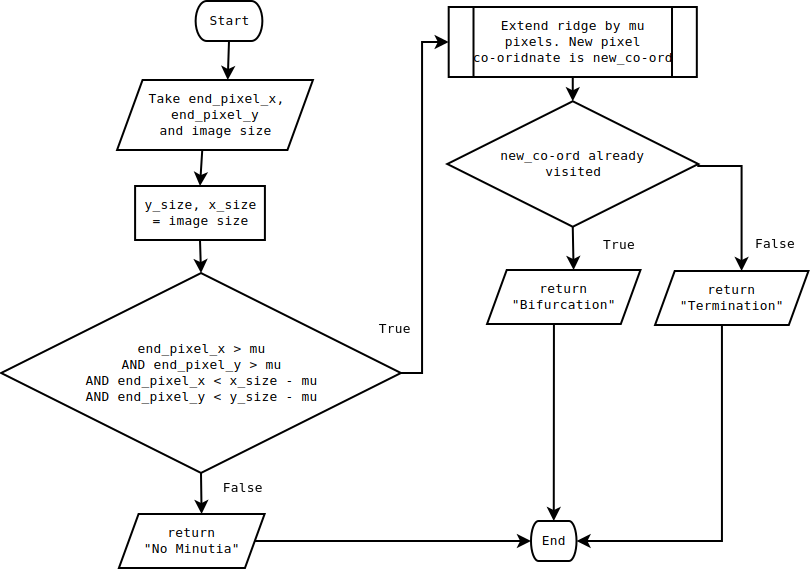
\includegraphics[width = \textwidth]{minutia}
          \caption{Flow chart for minutia detection. This is applied to the end of each ridge found.}
          \label{fig:min-alg}
        \end{figure*}

\section{Results \& Analysis}
	In order to test the various functions we use several images, shown in figure \ref{fig:ex_img}. Each of these images present their own challenges: \ref{fig:Example_curve_n0}, \ref{fig:Example_curve_n50} and \ref{fig:fingerprint5} all have quite wide ridges that plateau while \ref{fig:Example_curve_n50} and \ref{fig:arch} both have significant levels of noise that, if not properly dealt with, could easily lead to the ridge follower missing the true path of a ridge.

			\begin{figure*}
				\centering
				\subfloat[Simple wide curve.]{\label{fig:Example_curve_n0}
					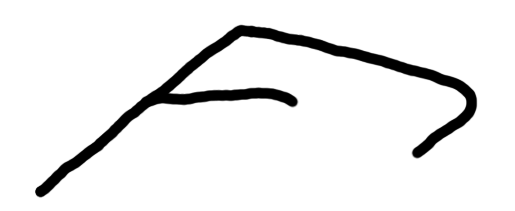
\includegraphics[width = 0.45\textwidth]{../Images/Example_curve_n0}} \qquad
				\subfloat[Simple wide curve with noise added.]{\label{fig:Example_curve_n50}
					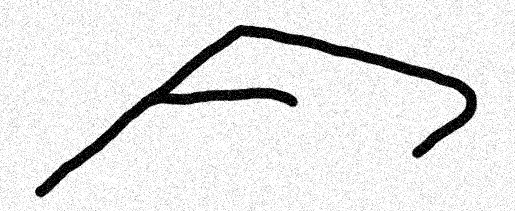
\includegraphics[width = 0.45\textwidth]{../Images/Example_curve_n50}} \\
				\subfloat[Scan of a real fingerprint.]{\label{fig:arch}
					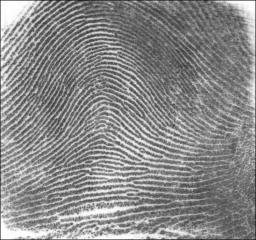
\includegraphics[width = 0.45\textwidth]{../Images/arch}}
\qquad
				\subfloat[Computer generated fingerprint.]{\label{fig:fingerprint5}
					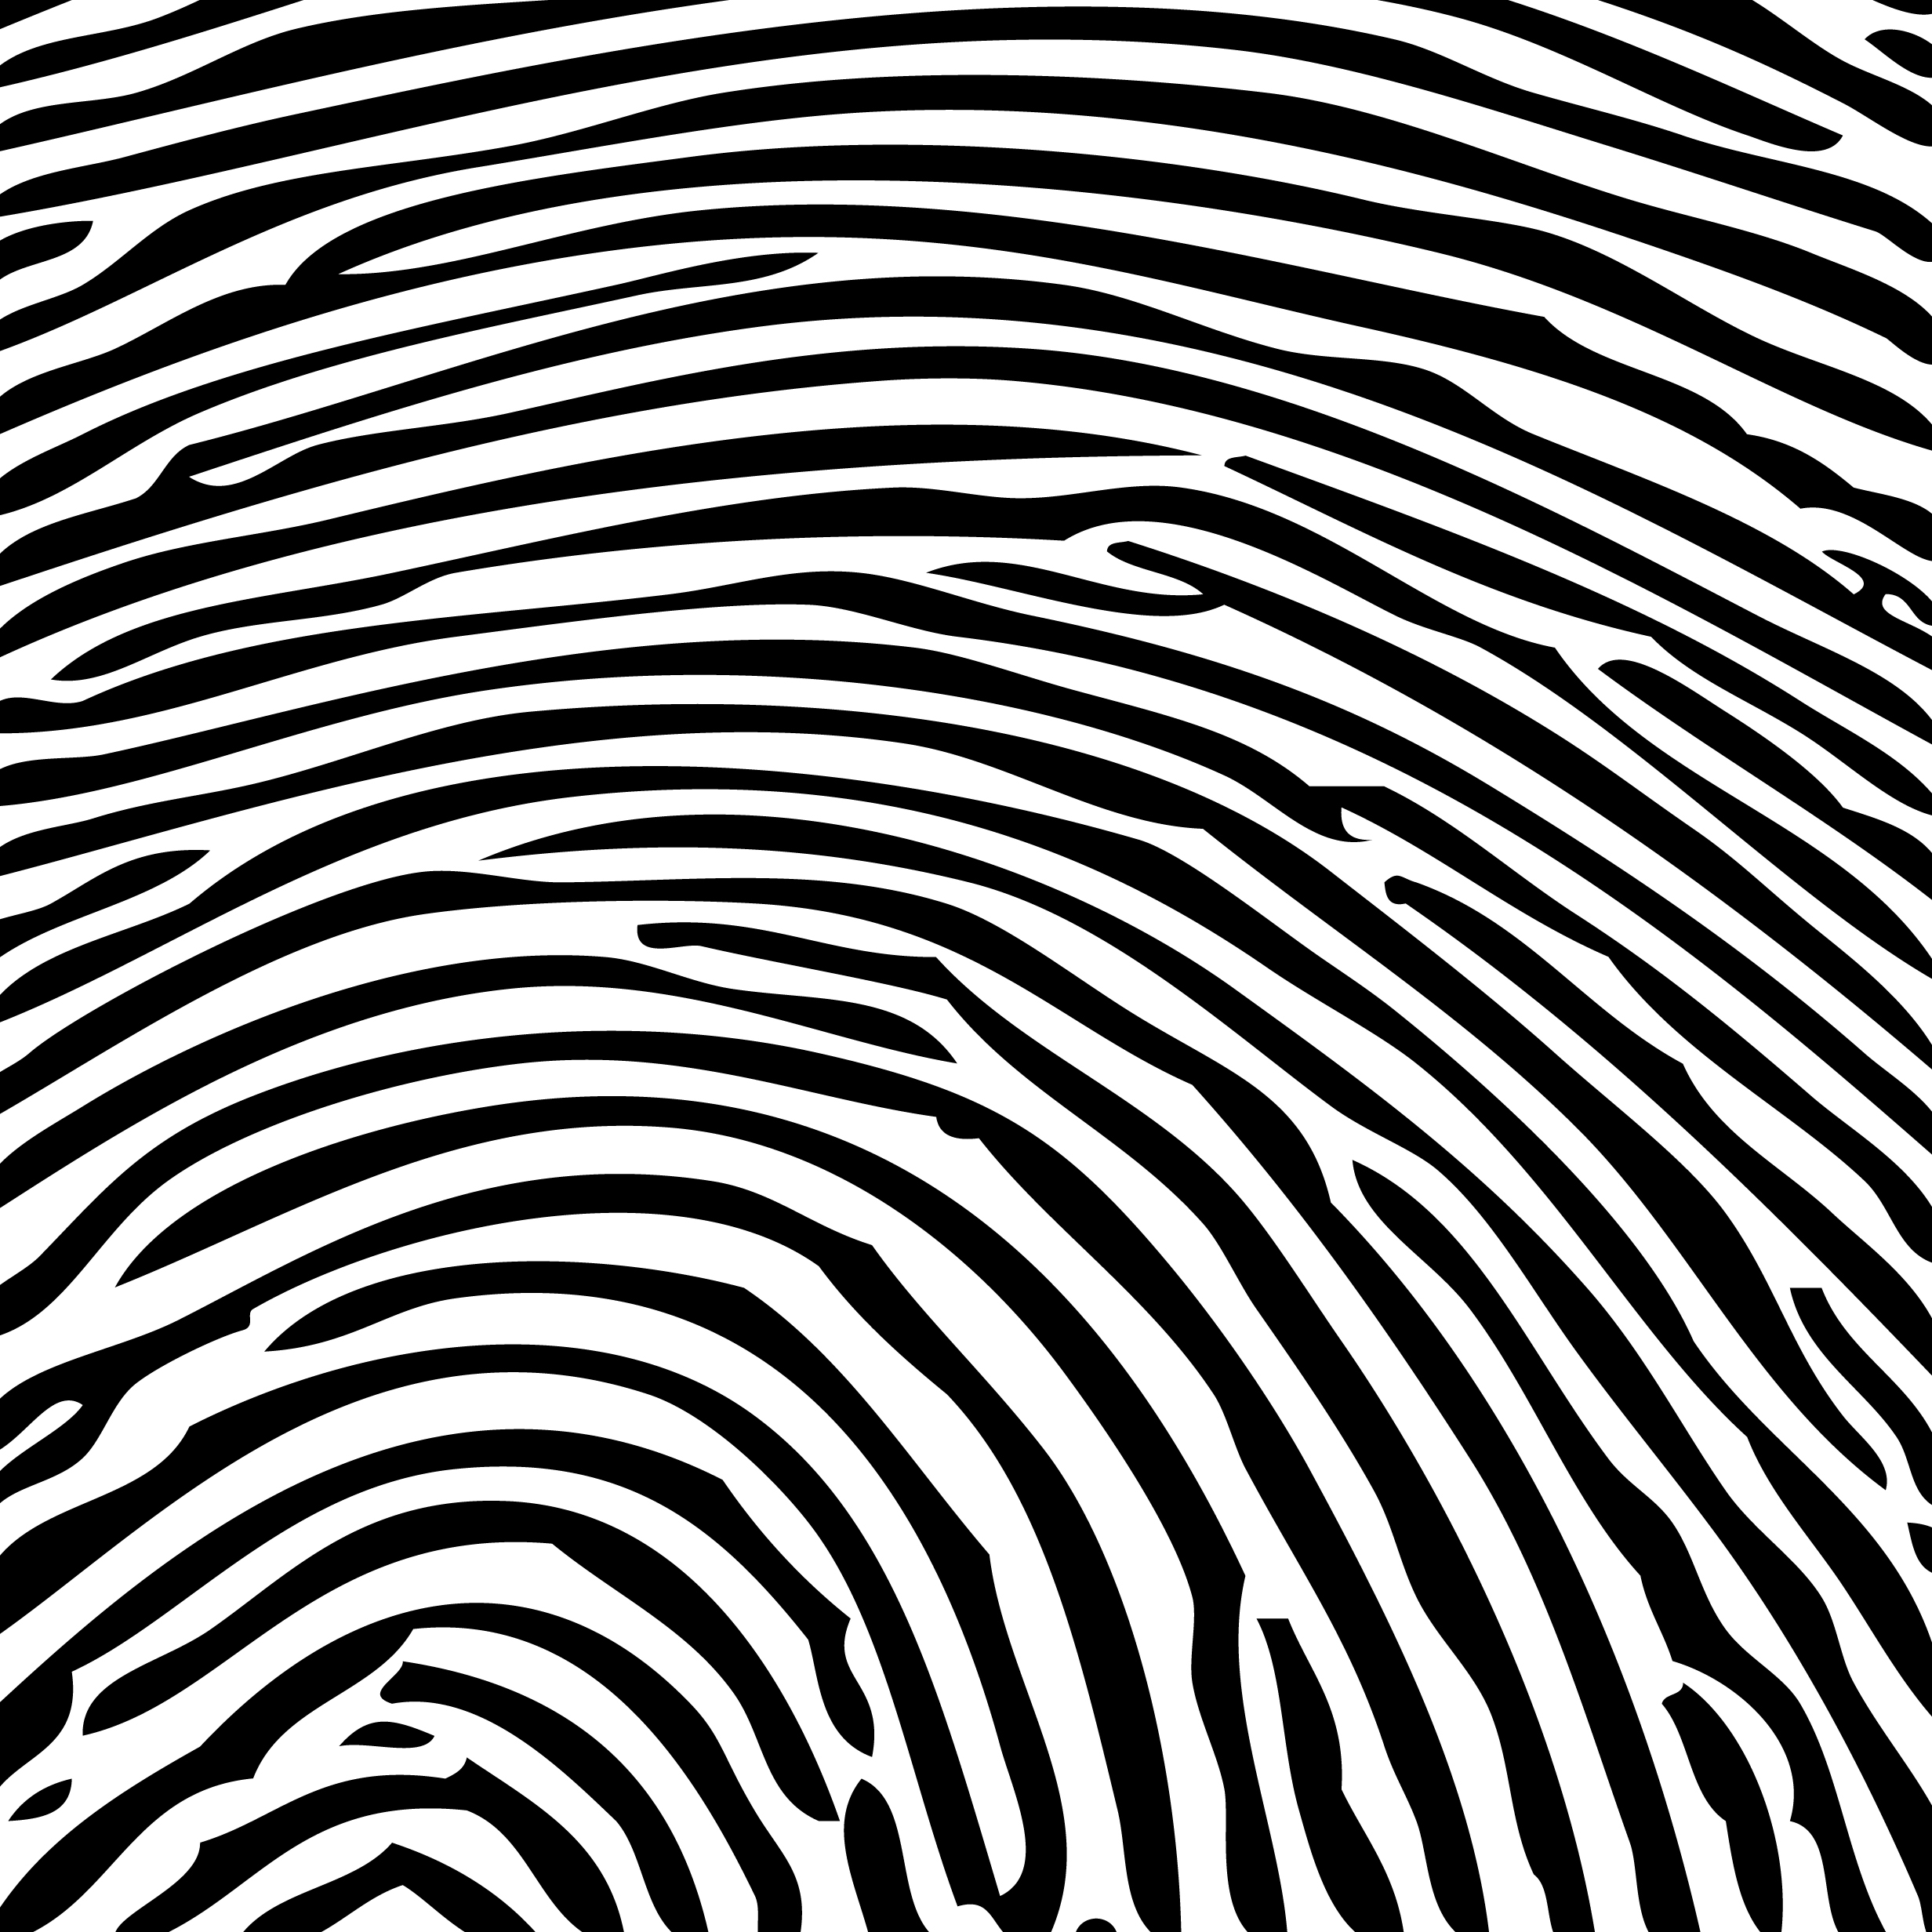
\includegraphics[width = 0.45\textwidth]{../Images/fingerprint5}}
				\caption{Example images used to test the functions written.}
				\label{fig:ex_img}
			\end{figure*}

	\subsection{The PND function}
			\begin{figure*}
				\centering
				\subfloat[Simple wide curve.]{\label{fig:PND_Example_curve_n0}
					\includegraphics[width = 0.48\textwidth]{PND_Example_curve_n0}} \;
				\subfloat[Simple wide curve with noise added.]{\label{fig:PND_Example_curve_n50}
					\includegraphics[width = 0.48\textwidth]{PND_Example_curve_n50}} \\
				\subfloat[Scan of a real fingerprint.]{\label{fig:PND_arch}
					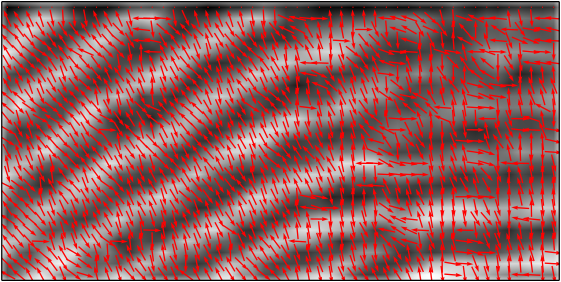
\includegraphics[width = 0.48\textwidth]{PND_arch}}
\;
				\subfloat[Computer generated fingerprint.]{\label{fig:PND_fingerprint5_small}
					\includegraphics[width = 0.48\textwidth]{PND_fingerprint5_small}}
				\caption{Sections of the example images after the PND function has been applied.}
				\label{fig:PND_img}
			\end{figure*}

		As can be seen in figures \ref{fig:PND_Example_curve_n0} and \ref{fig:PND_fingerprint5_small} the PND function does correctly calculate surface normals for a noise free image. It should be noted that in the system developed here black represents a low pixel value while white is high (as is standard for greyscale images), hence the normals point towards the black regions rather than away.

		If PND is applied to \ref{fig:Example_curve_n50} however, result is not as satisfactory (figure \ref{fig:PND_Example_curve_n50}). The point normals at the edge of the line do point towards the line however as the PND function has no way of smoothing out noise vectors scatter the image like mines in a playground\footnote{By which I mean that the mines are unwelcome and would maime children if not dealt with}. In the case of scan of a real fingerprint the noise does not seam to have been an issue. Some normals are incorrectly angled but most are pointing in the right direction.

		Overall it appears that on it's own the PND function can cope with some smudging and blurred images as long as the ridges are still present but cannot cope with white noise, especially if the image has sparse ridges and large monochromatic areas.

	\subsection{The ATD Function}
			\begin{figure*}
				\centering
				\subfloat[Simple wide curve.]{\label{fig:ATD_Example_curve_n0_5}
					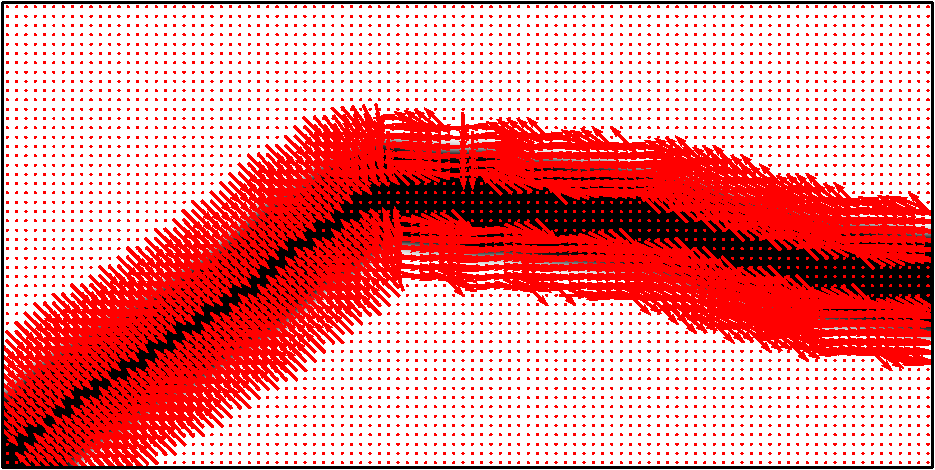
\includegraphics[width = 0.48\textwidth]{ATD_Example_curve_n0_5}} \;
				\subfloat[Simple wide curve with noise added.]{\label{fig:ATD_Example_curve_n50_5}
					\includegraphics[width = 0.48\textwidth]{ATD_Example_curve_n50_5}} \\
				\subfloat[Scan of a real fingerprint.]{\label{fig:ATD_arch_5}
					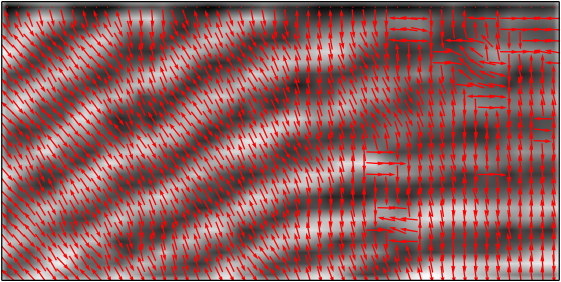
\includegraphics[width = 0.48\textwidth]{ATD_arch_5}}
\;
				\subfloat[Computer generated fingerprint.]{\label{fig:ATD_fingerprint5_small_5}
					\includegraphics[width = 0.48\textwidth]{ATD_fingerprint5_small_5}}
				\caption{Sections of the example images after the ATD function has been applied with a window size of 5.}
				\label{fig:ATD_img}
			\end{figure*}

		The results of the ATD function are not as encouraging as the PND results. Looking at figures \ref{fig:ATD_Example_curve_n0_5} and \ref{fig:ATD_fingerprint5_small_5} we can see that the function has spread the normals of the edges into regions that had no normal from the PND function (which is as expected) but most critically for certain sections the function calculates the direction of some of the vectors wrong. This appears to happen for sections that are nearly horizontal but is probably not due to the function incorrectly picking the case where $(u_1, u_2) = (0, 1)$, which can be seen the vectors pointing in opposing directions on opposite sides of the line. The bug may be due to a floating point error but at the time of writing the exact nature of the bug is unknown.

		For white noise the ATD function does not appear to help. Both the random noise normals and the actual edge normals have been merged, though a line correctly oriented normals does remain (ignoring the sections where the above mentioned malfunction occurs). For the real fingerprint the ATD function does seam to have improved the situation, with the normals in the blurred sections becoming properly oriented. If a larger window is used on this image, figure \ref{fig:ATD_arch_15}, one can see the effect of over smoothing the normals --- in the sections that are blurred the over smoothing had set all normals to the same direction. Setting the ATD window too large also appears to eliminate some of the ridges which again isn't surprising.

\begin{figurehere}
\centering
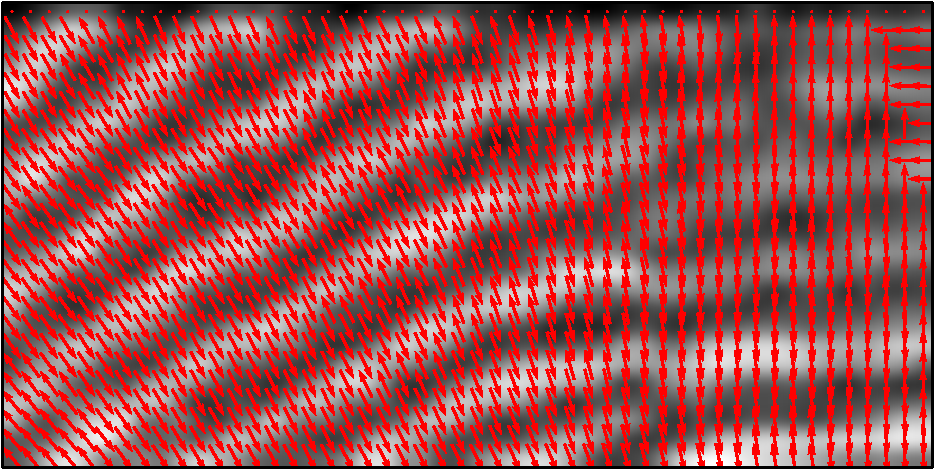
\includegraphics[width = 0.48\textwidth]{ATD_arch_15}
\caption{The result of applying the ATD function to the real fingerprint with window size of 15.}
\label{fig:ATD_arch_15}
\end{figurehere}

	\subsection{The Ridge Follower}
			\begin{figure*}
				\centering
				\subfloat[Path of the ridge follower.]{\label{fig:RF_arch}
					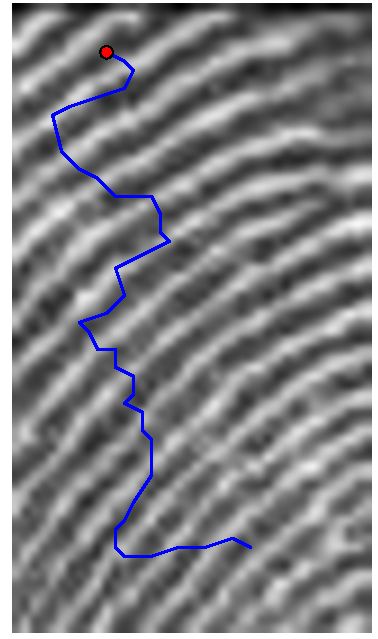
\includegraphics[width = 0.45\textwidth]{RF_arch}} \;
				\subfloat[Normals generated by ATD function.]{\label{fig:RF_ATD_arch}
					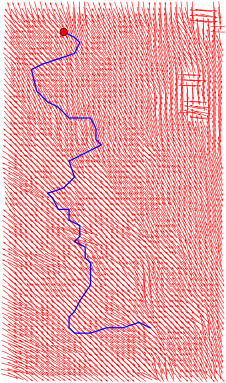
\includegraphics[width = 0.45\textwidth]{RF_ATD_arch}}
				\caption{Result of applying the ridge follower to the output of the ATD function ($\mu = 2$, $\sigma = 2$, ATD window size set to 5).}
				\label{fig:RF_img}
			\end{figure*}

		The results here are not encouraging - the ridge following algorithm, as implemented here, seams to switch between following a ridge and moving across ridges (figure \ref{fig:RF_arch}). This occurs independently of the previously mentioned bug in ATD (figure \ref{fig:RF_ATD_arch}). This problem may be down to how the function decides what the new value of $\phi_s$ is.

\section{Conclusion}
	A functioning system for computing the plane normal directions of a greyscale has been written and on testing was found to work well. This PND function has no way of dealing with noise hence a second function, the averaged tangent direction function, is necessary. On images with large uniform areas and white noise the ATD function is of little use however when tested with real fingerprints this is not a problem. It is found that when selecting the size of the window used by the ATD function it is important to not select a size that over smooths the normals.

	An attempt at implementing a ridge following algorithm was made however the attempt failed, in part because of the fault in the ATD function but also due to a flow in the way that the function calculates the direction it should go in.

\section{References}
\printbibliography[heading=none]
\end{multicols}

\appendix
\section{Code}
	\lstinputlisting[language=Python]{../basic_code_elements.py}

\end{document}
